\documentclass{beamer}

\title{Brancher AnyBlok à 14 ans d'historique métier}
\subtitle{Une histoire terrifiante de PHP, MySQL et MsSQL}
\author{Jean-Sébastien SUZANNE et Hugo QUEZADA}
\date{2 novembre 2019}

\newcommand{\TwitterLogo}{\protect
\includegraphics[height=
1.7ex,keepaspectratio]{./twitter.png}}
\newcommand{\EmailLogo}{\protect
\includegraphics[height=
1.7ex,keepaspectratio]{./email.png}}
\newcommand{\AnyBlokLogo}{\protect
\includegraphics[height=
1.7ex,keepaspectratio]{./anyblok.png}}

\usepackage{hyperref}
\usepackage{color}

\usetheme{Amsterdam}
\begin{document}
	\frame {
		\titlepage
	}
	
	\frame {
		\frametitle{Qui sommes nous ?}
		
		\begin{columns}
            \begin{column}{3cm}
                \begin{figure}
  					
\includegraphics[width=\linewidth]{logosensee-carre.jpg}
  					\label{fig:sensee}
				\end{figure}
			\end{column}
			\begin{column}{3cm}
				\begin{figure}
  					
\includegraphics[width=\linewidth]{lentillesmoinscheres-mobile.png}
  					\label{fig:lmc}
				\end{figure}
			\end{column}
		\end{columns} 			
		\begin{columns}
            \begin{column}{5cm}
                \textbf{\AnyBlokLogo{} Sébastien Suzanne}
		    	\begin{itemize}
			  		\item Répond aussi au nom de PAPABLOK
			  		\item \TwitterLogo{} @jssuzanne
			    	\item \EmailLogo{} js.suzanne@sensee.com
		    	\end{itemize}
			\end{column}
			\begin{column}{5cm}
				\textbf{Hugo Quezada}
		    	\begin{itemize}
			  		\item Dis le petit Basque du Chili
			  		\break
			    	\item \EmailLogo{} h.quezada@sensee.com
		    	\end{itemize}
			\end{column}
		\end{columns}
	}
	
	\frame{
		\frametitle{Existant}
		\framesubtitle{14 ans de code...}
		\begin{itemize}
			\pause
			\item Code legacy en PHP5 (pas de troll SVP)
			\item Pas de framework, beaucoup de code, très peu d'objet
			\break
			\pause
			\item Pas de tests
			\item Pas de CI
			\break
			\pause
			\item Pas d'ORM
		\end{itemize}
	}
	
	\frame{
		\frametitle{Existant}
		\framesubtitle{Une BdD un peu complexe...}
		\begin{itemize}
			\item  Schémas de base de données multiples
			\pause
			\item  Écosystème avec plusieurs SGBD (MySQL, MsSQL) souvent sans API
			\begin{figure}[p]
				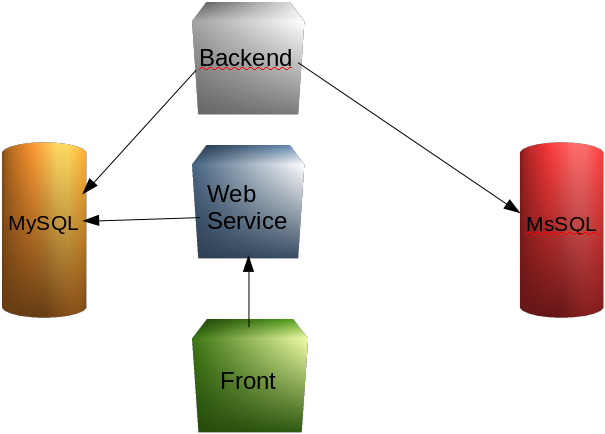
\includegraphics[height=25ex,keepaspectratio]{./schema_simplifie_lmc.png}
				\caption{Schéma simplifié}
			\end{figure}
		\end{itemize}
	}
	
	\frame{
		\frametitle{Vision finale}
		\framesubtitle{L'objectif}
		\begin{itemize}
		    \item Un code python propre et testé
			\item Une API simple et uniforme, utilisé dans tous nos projets
			\item Une application plus proche des standards actuels
			\item Un projet plus séduisant et plus attrayant pour des potentiels futurs développeurs 
		\end{itemize}
	}
	\frame{
		\frametitle{Vision finale}
		\framesubtitle{La stratégie}
		\begin{itemize}
			\item Modèle d'étranglement (Strangle pattern)
			\begin{figure}[p]
				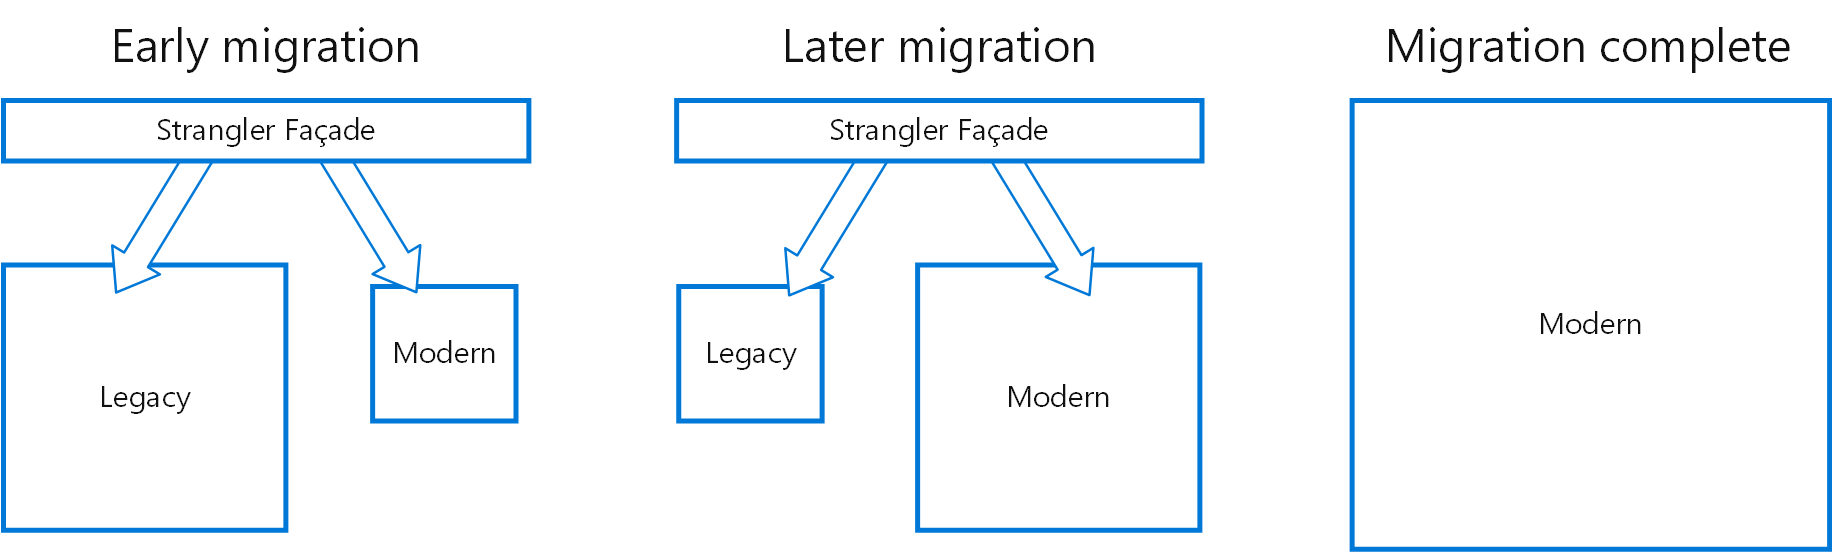
\includegraphics[height=15ex,keepaspectratio]{./strangler.png}
			\end{figure}
			\item Mapping des tables avec un nommage plus clair
			\item Développement piloté par les tests (TDD)
		\end{itemize}
	}
	\frame{
		\frametitle{Pourquoi avoir choisi AnyBlok ?}
		\framesubtitle{AnyBlok: Présentation}
		\begin{itemize}
		\item Python 3.6 et plus
		\item MPL2
		\item PyPi
		\item Modulaire
		\item Dépendances fiables (SQLAlchemy, Alembic, ...)
		\item Possibilité de reprendre une base existante.
		\end{itemize}
	}
	\frame{
		\frametitle{Pourquoi avoir choisi AnyBlok ?}
		\framesubtitle{AnyBlok: Structure}
		\begin{figure}
  			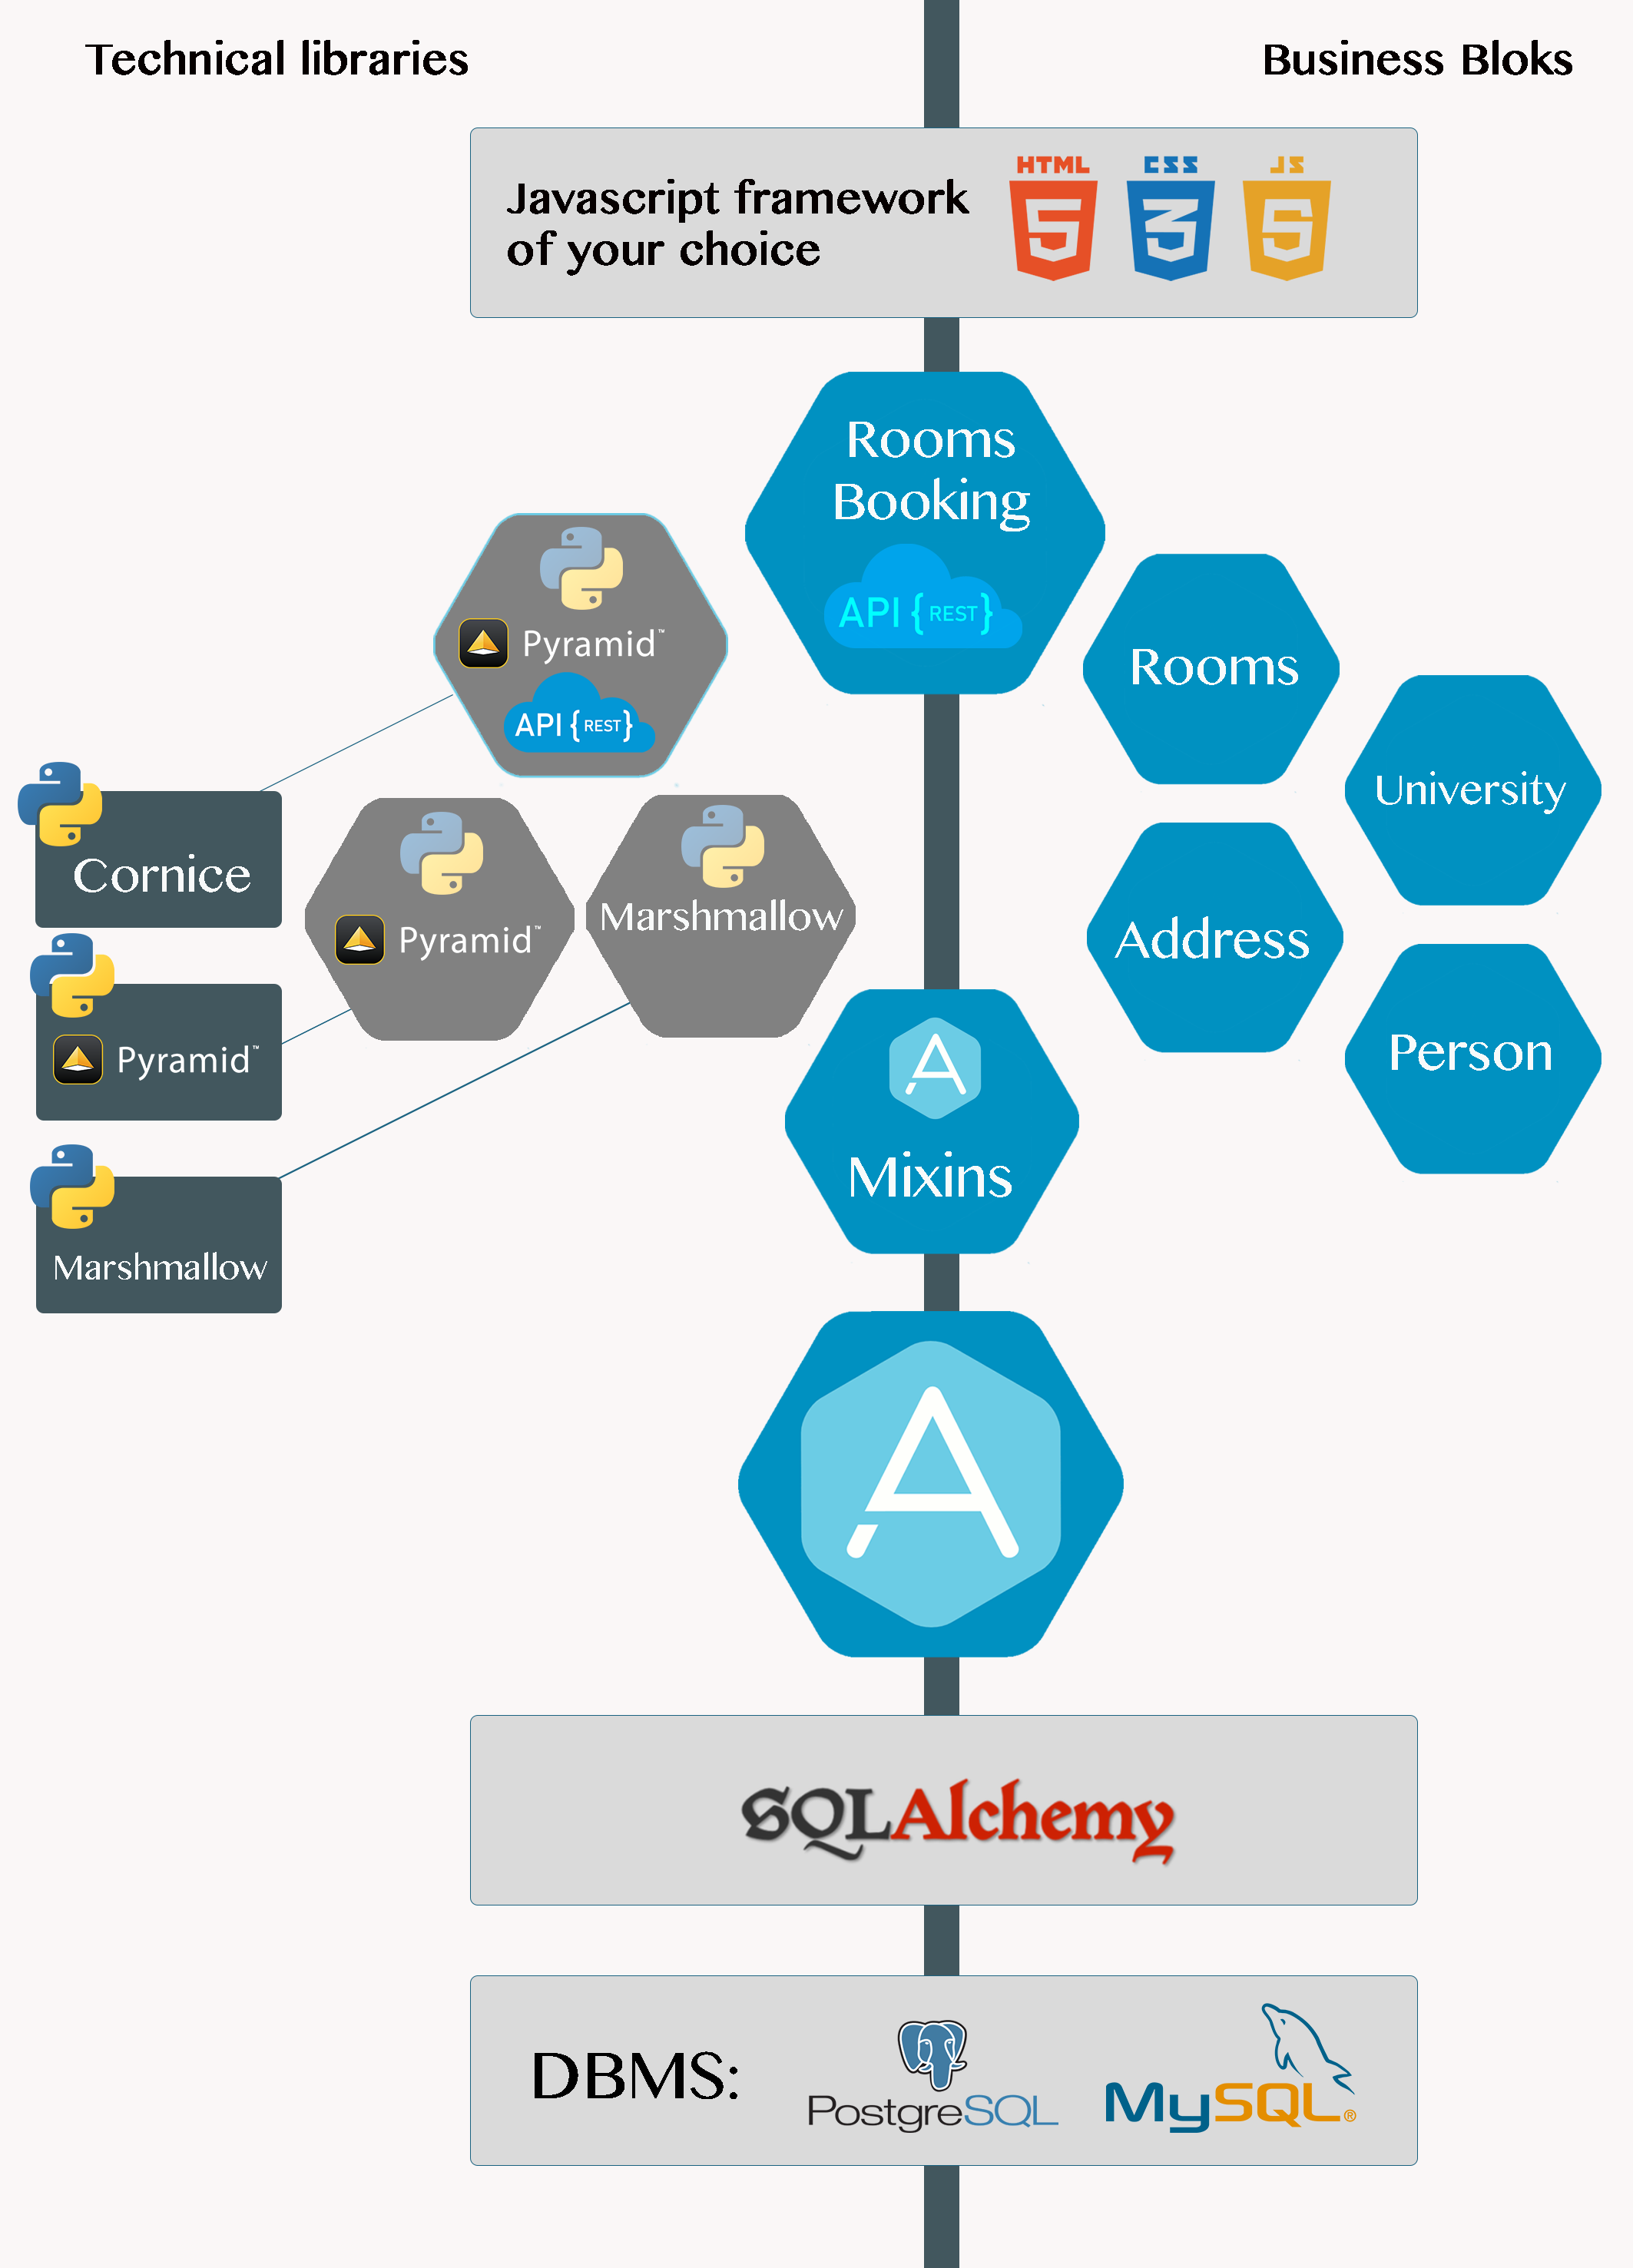
\includegraphics[height=42ex,keepaspectratio]{bloks_dependencies.png}
  			\label{fig:test unitaire}
		\end{figure}
	}
	\frame{
		\frametitle{Pourquoi avoir choisi AnyBlok ?}
		\framesubtitle{AnyBlok: Écrire des tests pour notre Model}
		\begin{figure}
  			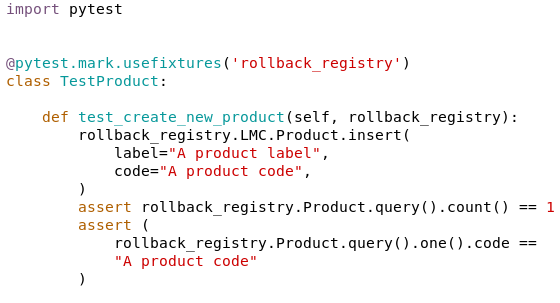
\includegraphics[width=\linewidth]{testU.png}
  			\label{fig:test unitaire}
		\end{figure}
	}
	\frame{
		\frametitle{Pourquoi avoir choisi AnyBlok ?}
		\framesubtitle{AnyBlok: Définir le Model}
		\begin{figure}
  			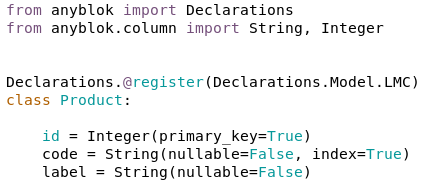
\includegraphics[width=\linewidth]{model1.png}
  			\label{fig:Model 1}
		\end{figure}
	}
	\frame{
		\frametitle{Pourquoi avoir choisi AnyBlok ?}
		\framesubtitle{AnyBlok: Définir un Model sur une table existante}
		\begin{figure}
  			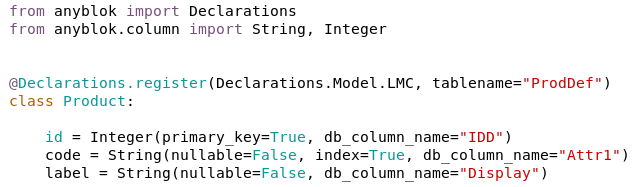
\includegraphics[width=\linewidth]{model2.png}
  			\label{fig:Model 2}
		\end{figure}
	}
		\frame{
		\frametitle{Pourquoi avoir choisi AnyBlok ?}
		\framesubtitle{AnyBlok: Écrire des tests pour notre L'API}
		\begin{figure}
  			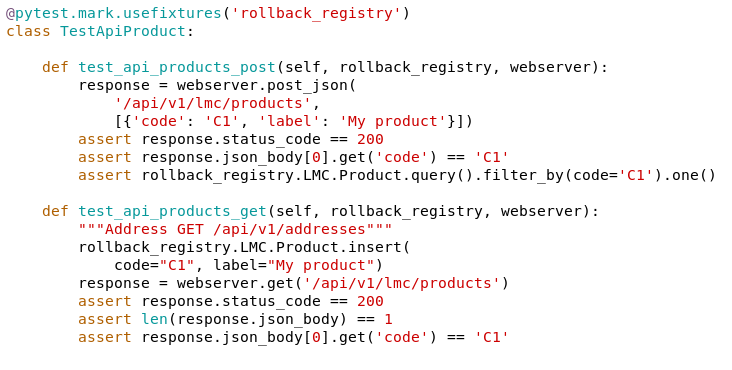
\includegraphics[width=\linewidth]{apitestU.png}
  			\label{fig:test unitaire API}
		\end{figure}
	}
	\frame{
		\frametitle{Pourquoi avoir choisi AnyBlok ?}
		\framesubtitle{AnyBlok: Écrire une API rest}
		\begin{figure}
  			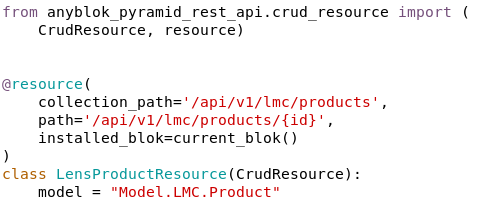
\includegraphics[width=\linewidth]{api.png}
  			\label{fig: API}
		\end{figure}
	}
	
	\frame{
		\frametitle{Evolutions et intégrations dans AnyBlok}
		\framesubtitle{Compatibilité avec MySQL}
		
		\pause
		\begin{itemize}
			\item Deux semaines de travail
			\item Beaucoup de recherches et d'incompréhensions 
		\end{itemize}
	}	
	\frame{
		\frametitle{Evolutions et intégrations dans AnyBlok}
		\framesubtitle{Compatibilité avec MySQL : Les tests unitaires}
		
		\begin{itemize}
			\item Mise à jour de la configuration Travis-CI
			\item Activer le mode transactionnel de innoDB
			\item {\color{blue}\href{https://dev.mysql.com/doc/refman/8.0/en/implicit-commit.html}{Les commits implicites}}
		\end{itemize}
	}	
	\frame{
		\frametitle{Evolutions et intégrations dans AnyBlok}
		\framesubtitle{Compatibilité avec MySQL : Limitations}
		
		\begin{itemize}
			\item Pas de Python 3.5
			\item Pas de CheckConstraint et autre contrainte exclusive à PostgreSQL
			\item Datetime naïves
			\item Pas de chiffrement sur les colonnes de type UUID
			\item Pas de véritable Booléen
		\end{itemize}
	}	
	\frame{
		\frametitle{Evolutions et intégrations dans AnyBlok}
		\framesubtitle{Compatibilité avec MariaDB : Limitations }
		
		\begin{itemize}
			\item Pas de Python 3.5
			\item Pas de CheckConstraint et autre contrainte exclusive à PostgreSQL
			\item Datetime naïves
			\item Pas de chiffrement sur les colonnes UUID
			\item Pas de véritable Booléen
			\item \pause Taille des clés primaires plus petite
			\item Pas de colonnes JSON
		\end{itemize}
	}
	\frame{
		\frametitle{Évolutions et intégrations dans AnyBlok}
		\framesubtitle{Compatibilité avec MsSQL : Limitations}
		
		\begin{itemize}
			\item Pas de Python 3.5
			\item Pas de CheckConstraint et autre contrainte exclusive à PostgreSQL
			\item \pause Lent... Très très lent...
		\end{itemize}
	}
	\frame{
		\frametitle{Évolutions et intégrations dans AnyBlok}
		\framesubtitle{Définition de schémas}
		\begin{itemize}
			\item Programmatique ou par configuration
			\item Poser sur un modèle ou un namespace
			\item Ajout de suffixes ou préfixes pour les tests
		\end{itemize}
		\hfill \linebreak
		\pause Problématiques
		\begin{itemize}
			\item génération de foreign key
			\item migration
		\end{itemize}
	}
	\frame{
		\frametitle{Évolutions et intégrations dans AnyBlok}
		\framesubtitle{Ajouter un schema a un Model}
		Dans Le Model
		\begin{figure}
  			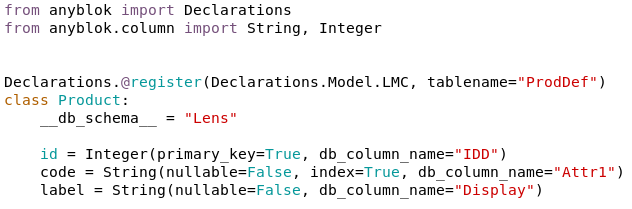
\includegraphics[width=\linewidth]{schema.png}
  			\label{fig:Model avec un schema}
		\end{figure}
		Par la configuration
		\begin{figure}
  			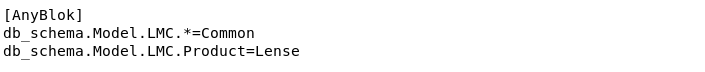
\includegraphics[width=\linewidth]{schema2.png}
  			\label{fig:Schema depuis la conf}
		\end{figure}
	
	}
	\frame{
		\frametitle{Interface Graphique}
		\framesubtitle{FuretUI}
		\begin{figure}

  			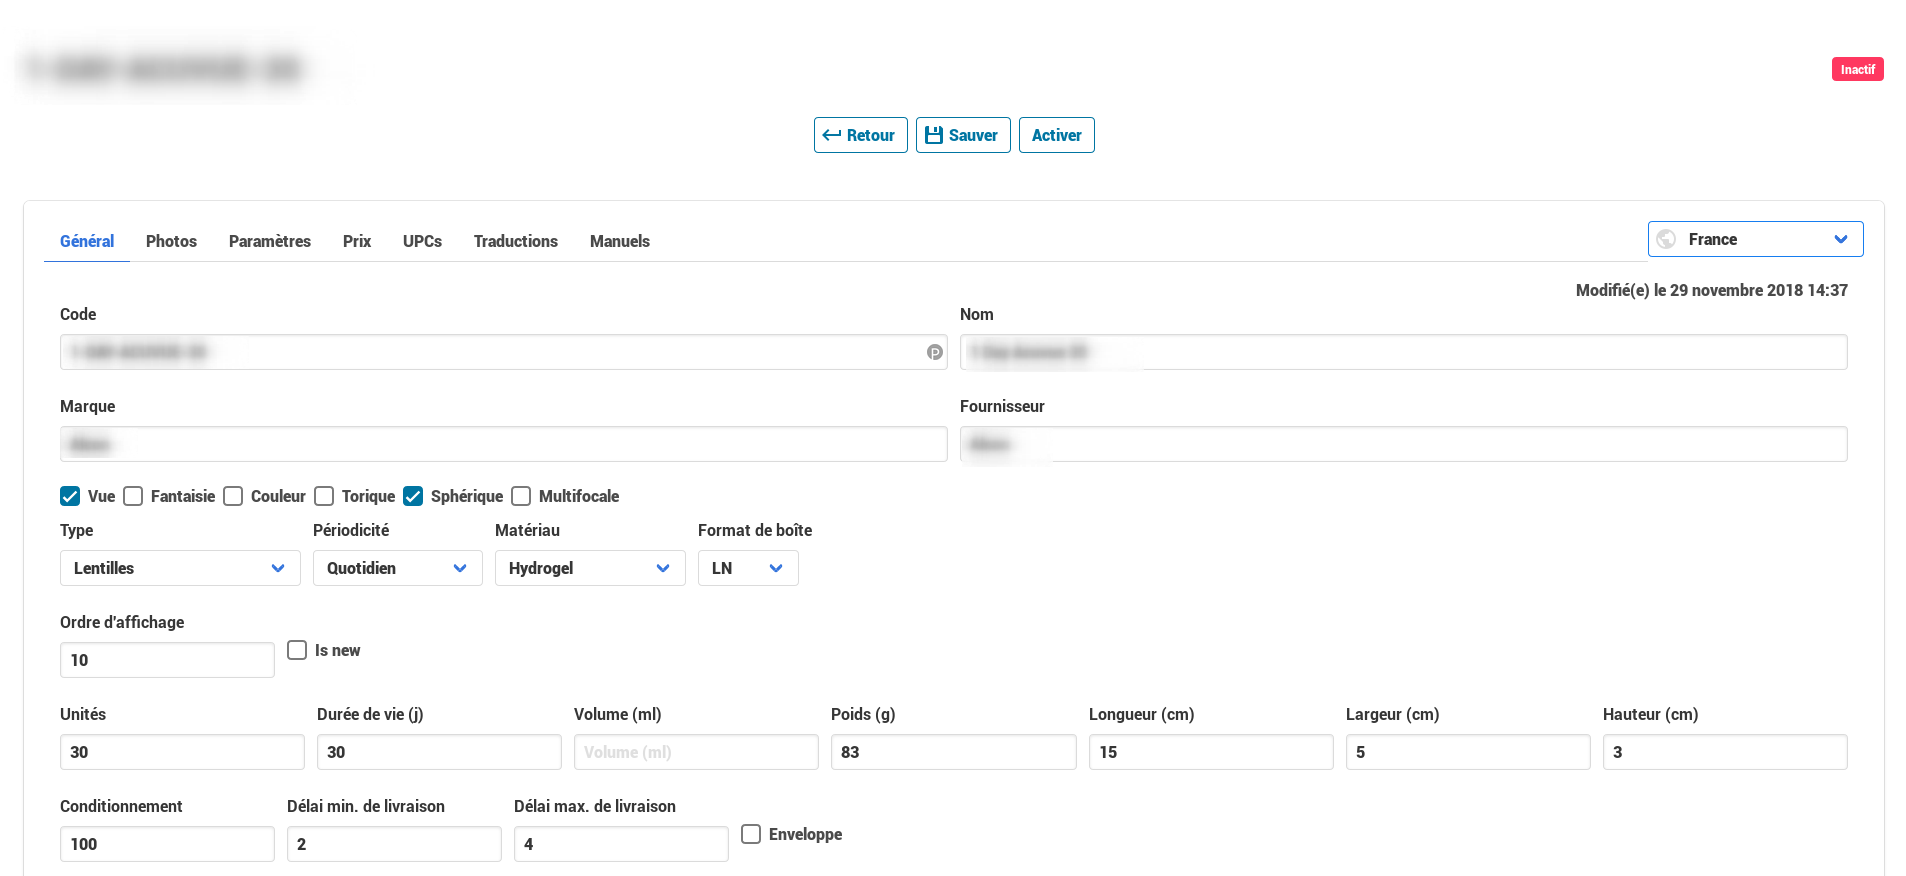
\includegraphics[width=\linewidth]{exemple_furetui_produits.png}
  			\label{fig: FuretUI List}
		\end{figure}
	}
	\frame{
		\frametitle{Interface Graphique}
		\framesubtitle{FuretUI}
		\begin{figure}
  			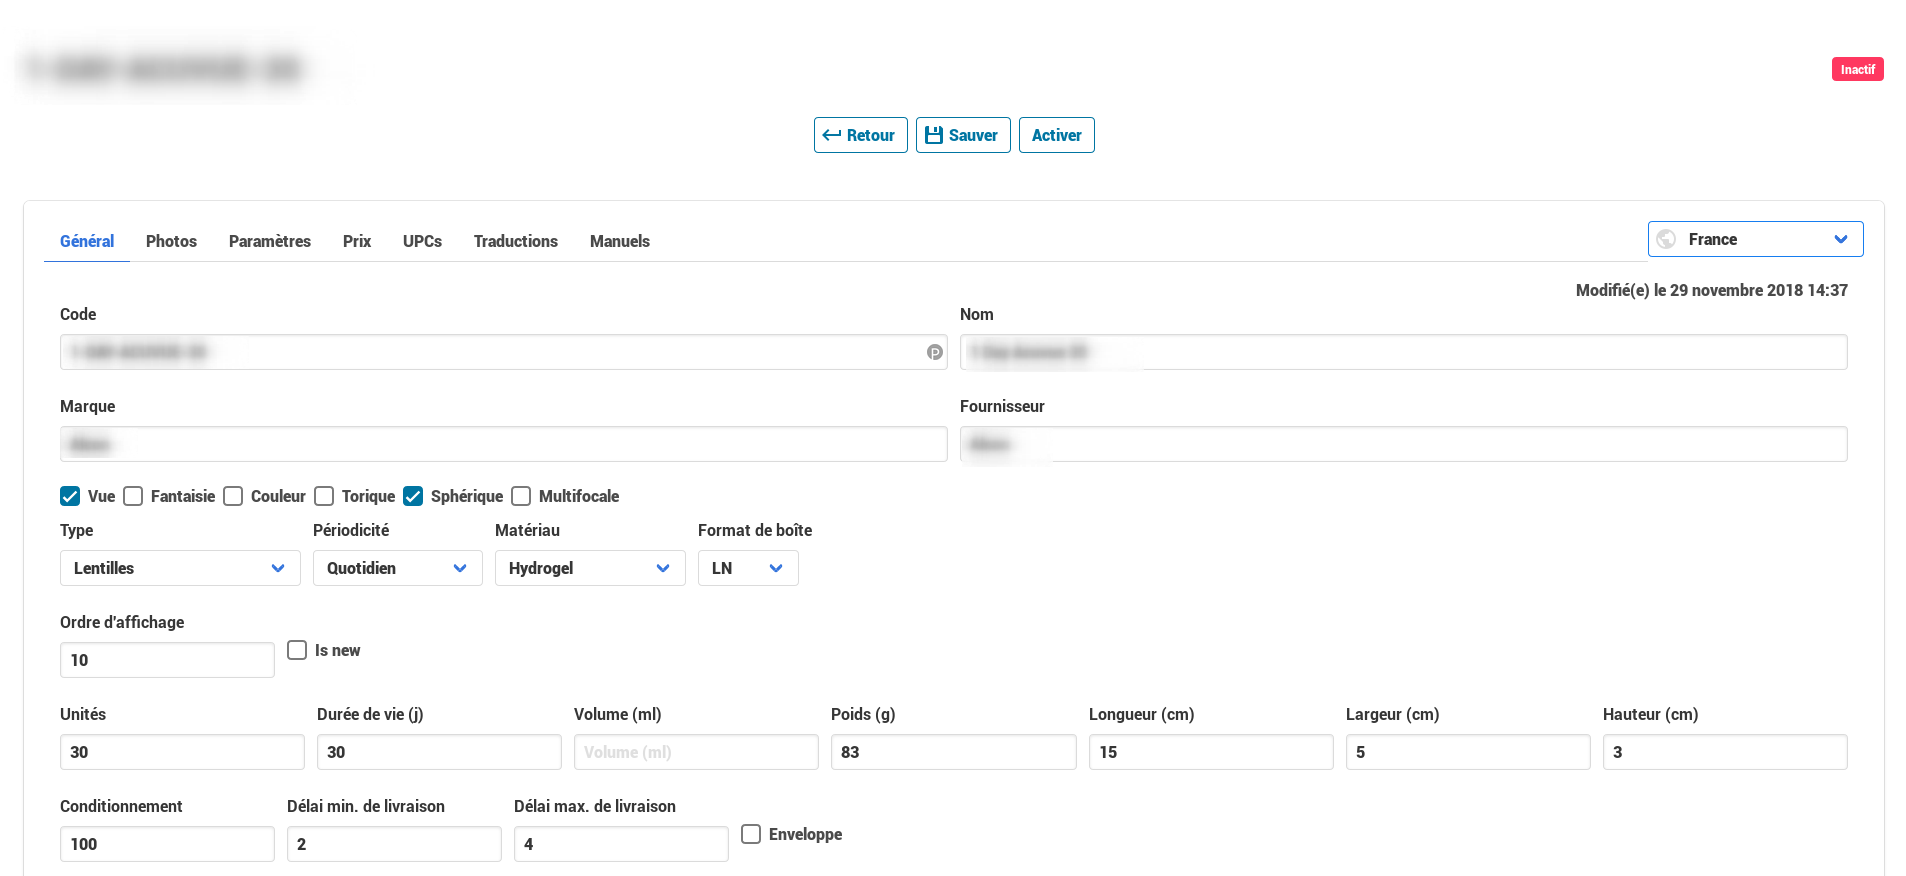
\includegraphics[width=\linewidth]{exemple_furetui_produits_page.png}
  			\label{fig: FuretUI Page}
		\end{figure}
	}
	\frame{
		\frametitle{AnyBlok}
		\framesubtitle{Documentation}
		\begin{itemize}
		\item https://anyblok.gitbooks.io/anyblok-book/content/en/
		\item doc.anyblok.org
		\item https://github.com/AnyBlok
		\item https://gitter.im/AnyBlok/community
		\end{itemize}
	}
	\frame{
		\frametitle{Fin}
		\begin{columns}
			\begin{column}{4cm}
			\end{column}
			\begin{column}{8cm}
				Des questions ? 
				\break
				Des remarques ?
			\end{column}
		\end{columns}
	}
		
\end{document}
